\subsection*{Defining dependencies}
The database must respect dependencies between data elements and prevent incomplete, orphaned, or mismatched data.
DataJoint facilitates setting, enforcing, and displaying data dependencies. 
The edges of the graph in the entity relationship diagram (ERD) in Fig.\ \ref{schema}\,B denote dependencies directed downward: relations below are dependent on relations above when connected.
Chains of dependencies effectively set the order in which  data must be populated. 
Thus the ERD serves as an effective communication tool for the overall data organization and the sequence of steps to be followed for data entry and  processing.
Each base relation can depend on multiple other relations but the dependency graph must be acyclic: a relation cannot depend on itself or on other relations that depend on it directly or through other relations.

To create a dependency, the dependent relation's data definition must include the line \matlab{-> Reference}, where \matlab{Reference} is the class name of the referenced base relation.

Setting a dependency has two effects:
\begin{enumerate}[(a)]
\item the primary key attributes of the referenced relation are copied into the definition 
\item a foreign key constraint is created to the referenced relation.
\end{enumerate}

The foreign key constraint causes the database to reject any new tuple in the dependent relation unless there exists a matching tuple in the referenced relation. 
Conversely, deleting a tuple from the referenced relation will cause all matching tuples in all the dependent relations to be deleted too.

For example, when \matlab{Session} depends on \matlab{Animal} (Fig.\ \ref{schema}\,B),
\matlab{Animal}'s primary key attribute {\tt animal} is automatically included in \matlab{Session}'s heading (Fig.\ \ref{schema}\,C and D). 
A new session cannot be entered for an animal that has not yet been entered;  and when an animal is deleted, all its sessions will be  deleted as well, along with all the dependent data below in the hierarchy.

Importantly, DataJoint treats tuples in relations as indivisible; dependencies are established between whole tuples rather than between attribute values.
DataJoint methods modify relations only by inserting or deleting entire tuples and cannot update individual attribute values independently.

Such discipline guarantees that any changes of attribute values will trigger recomputation of all dependent data. 
Of course, users can deliberately intervene and modify values manually to bypass dependencies when necessary, provided that they have been granted update privileges by the database administrator.

The primary keys and dependencies between base relations allow defining a rich variety of relationships between data elements.  
Three common types of relationships illustrate this point (Figure \ref{dep}). 

\begin{figure*}[h]
\begin{center}
\begin{tabular}{p{0.2\textwidth}p{0.2\textwidth}p{0.4\textwidth}}
{\sf \large A} &
{\sf \large B} &
{\sf \large C} \\
\vspace{0pt} 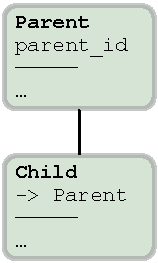
\includegraphics{./figures/depA.pdf} &
\vspace{0pt} 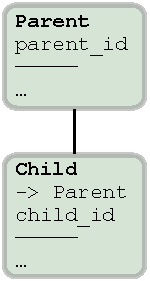
\includegraphics{./figures/depB.pdf} &
\vspace{0pt} 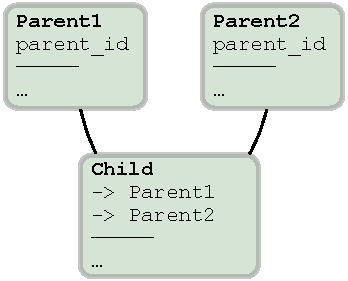
\includegraphics{./figures/depC.pdf}
\end{tabular}
\end{center}
\caption{
{\bf Three common replationships defined through the dependencies and primary keys of base relations.}
{\sf A.} A one-to-one relationship.
{\sf B.} A one-to-many (hierarchical) relationship.
{\sf C.} A combinatorial relationship. 
}
\label{dep}
\end{figure*}


\begin{itemize}
\item
In a one-to-one relationship (Fig.\ \ref{dep}\,A), relation \matlab{Child} declares a dependency within its primary key on \matlab{Parent} but does not add any new attributes to its primary key.
Thus the primary key for \matlab{Child} is the same as for \matlab{Parent}: only one tuple in \matlab{Child} can exists for each tuple in \matlab{Parent}.
\item
In a one-to-many relationship (Fig.\ \ref{dep}\,B), relation \matlab{Child} declares a dependency within its primary on \matlab{Parent} but also declares an additional attribute \matlab{child_id} in its primary key, which allows \matlab{Child} to have multiple tuples matching each tuple in \matlab{Parent}.
\item
In a combinatorial relationship (Fig.\ \ref{dep}\,C), relation \matlab{Child} declares a dependency within its primary key on  multiple relations.
In this example, \matlab{Child}'s primary key combines the primary key attributes from both \matlab{Parent1} and \matlab{Parent2}.  
This means that \matlab{Child} holds tuples corresponding to any combination of tuples in \matlab{Parent1} and \matlab{Parent2}.
\end{itemize}
Examples of other types of relationships may be found in the online resources.
